\begin{ledgroupsized}[r]{120mm}
\footnotesize 
\pstart
\noindent
\textbf{\"{U}berlieferung:}
\pend
\end{ledgroupsized}
\begin{ledgroupsized}[r]{114mm}
\footnotesize 
\pstart
\parindent -6mm
\makebox[6mm][l]{\textit{L}}Konzept: LH XXXVII 4 Bl. 61-62. 1 Bog. 2\textsuperscript{o}, Bl. 62 um die unteren \nicefrac{2}{3} beschnitten. 2 \nicefrac{1}{3} S. Bl. 62~v\textsuperscript{o} leer. Ein Wasserzeichen auf Bl.~61. Dort auch Textverluste durch Papierabbrüche am Rand.
Textträger durch Papiererhaltungs\-ma{\ss}nahmen gesichert. \\Cc 2, Nr. 1504
\pend
\end{ledgroupsized}
%
%\normalsize
\vspace*{5mm}
\begin{ledgroup}
\footnotesize 
\pstart
\noindent
\footnotesize{\textbf{Datierungsgr\"{u}nde}: Das Wasserzeichen ist für die Monate Februar bis September 1676 belegt.}
\pend
\end{ledgroup}
%%%%
%%%%
\vspace*{8mm}
\count\Bfootins=1000
\pstart 
\normalsize
\noindent
[61~r\textsuperscript{o}]
Aeque facile est corpora disposita in arcu $\displaystyle BC$ sursum attollere
\edtext{circa centrum $\displaystyle\langle A \rangle$}{\lemma{circa centrum $\displaystyle\langle A \rangle$}\Bfootnote{\textit{erg. L}}},
quam corpora aequalia disposita in recta $\displaystyle EF$. quia idem corpus pendulum\protect\index{Sachverzeichnis}{pendulum} $\displaystyle AD$ ex $\displaystyle D$ 
veniens in $\displaystyle C$, ipsum arcum
\edtext{$\displaystyle BC$ cum suis globis transferet in $\displaystyle GL$,}{\lemma{$\displaystyle BC$}\Bfootnote{%
\textit{(1)}\ cum chordis connexis transferet in arcum
\textit{(2)}\ cum [...] $\displaystyle GL$,
\textit{L}}}
quantum praecise satis est, ut corpus $\displaystyle B$ elevatum
in $\displaystyle G$ possit currere in $\displaystyle D$, eademque continuare;
et \edtext{idem $\displaystyle D$, si ex eadem altitudine pervenisset in}{\lemma{idem}\Bfootnote{%
\textit{(1)}\ pendulum\protect\index{Sachverzeichnis}{pendulum} $\displaystyle GD$ si in
\textit{(2)}\ $\displaystyle D$, si [...] pervenisset in
\textit{L}}}
[$\displaystyle MN$]\edtext{}{\Bfootnote{$\displaystyle M$ \textit{\ L \"{a}ndert Hrsg.}}},
[rectam]\edtext{}{\Bfootnote{recta \textit{\ L \"{a}ndert Hrsg.}}},
utique eandem in fine vim habet, eandem scilicet\protect\index{Sachverzeichnis}{velocitas}%
\textso{ velocitatem et }\edtext{\textso{molem.}\protect\index{Sachverzeichnis}{molis} Et}{\lemma{\textso{molem.}}\Bfootnote{%
\textit{(1)}\ Ergo
\textit{(2)}\ Et
\textit{L}}}
idem tunc incidens in $\displaystyle MN$ et funem\protect\index{Sachverzeichnis}{funis}
[$\displaystyle NPF$]\edtext{}{\Bfootnote{$\displaystyle MPF$ \textit{\ L \"{a}ndert Hrsg.}}}
circa trochleam\protect\index{Sachverzeichnis}{trochlea} $\displaystyle P$ replicatum trahens[,]
etiam elevabit $\displaystyle FE$ in $\displaystyle HQ$. quae autem
\edtext{ab eadem causa\protect\index{Sachverzeichnis}{causa} praecise fieri possunt aequalia sunt}{\lemma{ab}\Bfootnote{%
\textit{(1)}\ eodem proveniunt effectu\protect\index{Sachverzeichnis}{effectus} aequalia sunt
\textit{(2)}\ eadem [...] sunt
\textit{L}}},
par ergo est difficultas illa quam haec elevare,
quod et aliunde constat. Ex natura scilicet plani inclinati\protect\index{Sachverzeichnis}{planum inclinatum}.
Et ex his etiam forte supposito jam plano inclinato\protect\index{Sachverzeichnis}{planum inclinatum},
contraria ratione demonstrari poterit principium nostrum.
Necesse est enim tantundem attolli posse
utcunque inclinatio\protect\index{Sachverzeichnis}{inclinatio} in plano curvaque superficie
inter easdem parallelas disposita.
Sed dubito an nostra hinc possint demonstrari.
\pend
\pstart
Corpus \edtext{$\displaystyle B$}{\lemma{$\displaystyle B$}\Bfootnote{\textit{erg. L}}}
in superficie inclinata $\displaystyle BC$
descendens et in recta $\displaystyle CD$ procurrens,
impingit in seriem \edtext{corporum in $\displaystyle DE$ arcu}{\lemma{corporum}\Bfootnote{\textbar\ in \textit{erg.} \textbar\ $\displaystyle DE$ arcu \textit{L}}} aliquo vel superficie dispositorum
eamque elevat in $\displaystyle FG$.
Ajo si contra catena\protect\index{Sachverzeichnis}{catena} fuisset in $\displaystyle FG$,
et descendisset in $\displaystyle ED$.
eodemque momento corpus [$\displaystyle B$]\edtext{}{\Bfootnote{$\displaystyle BC$ \textit{\ L \"{a}ndert Hrsg.}}}
emenso spatio $\displaystyle BCD$
in $\displaystyle D$ occurrisset,
fuisset aequilibrium virium\protect\index{Sachverzeichnis}{aequilibrium virium}.
Nam tanta est vis unaquaeque, quanta est vis
\edtext{tota}{\lemma{tota}\Bfootnote{\textit{erg. L}}}
quam produxit.
(Res tantum distinctius explicanda.)
Imo quod elegantissimum idem erit,
semperque erit aequilibrium\protect\index{Sachverzeichnis}{aequilibrium},
ubicunque alio in loco sibi occurrant,
ut si catena\protect\index{Sachverzeichnis}{catena}
\edtext{ejusmodi $\displaystyle GF$ per $\displaystyle ED$, eat usque in}{\lemma{ejusmodi}\Bfootnote{%
\textit{(1)}\ reascendat usque in
\textit{(2)}\ $\displaystyle GF$ [...] usque in
\textit{L}}}
$\displaystyle M$, et ibi occurrat eidem
\pend
%\vspace*{1em}
\pstart
\noindent
\centering
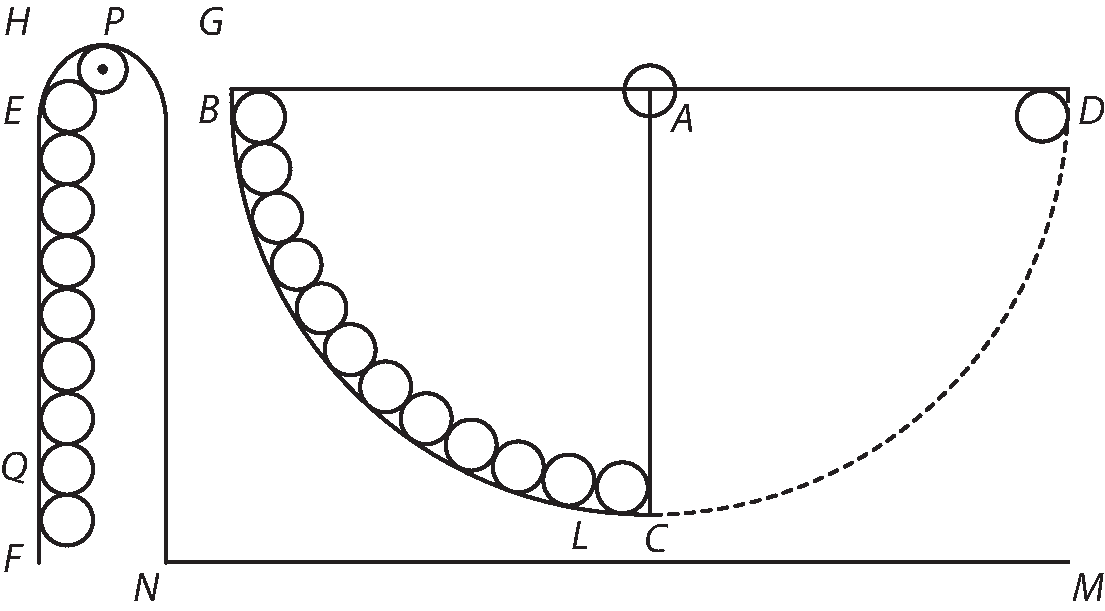
\includegraphics[trim = 0mm -3mm 0mm 0mm, clip, width=0.76\textwidth]{images/LH037,04_061r-d1.pdf}\\
\noindent \centering [\textit{Fig. 1}] 
\pend
\vspace{2em}
\pstart \noindent corpori \setline{1}$\displaystyle B$
ex $\displaystyle B$ in $\displaystyle M$ eodem tempore venienti[,]
rursus erit aequilibrium\protect\index{Sachverzeichnis}{aequilibrium},
(modo scilicet descensus\protect\index{Sachverzeichnis}{descensus} ejus non fuerit major quam ex altitudine $\displaystyle GE$)
idem erit, etsi tota catena\protect\index{Sachverzeichnis}{catena} in unam massam\protect\index{Sachverzeichnis}{massa} collecta,
et ex suae gravitatis centro\protect\index{Sachverzeichnis}{centrum gravitatis} suspensa intelligatur.
\pend
\pstart
Demonstrandum est generaliter,
quod in his quoque sufficiat consideratio centri gravitatis\protect\index{Sachverzeichnis}{centrum gravitatis},
seu quod corpus eandem vim habeat,
etsi omne ejus pondus\protect\index{Sachverzeichnis}{pondus} in centrum gravitatis\protect\index{Sachverzeichnis}{centrum gravitatis} sit collectum.
Et generaliter in quantamcunque licet exiguitatem.
Quod dixi nihil referre, ubi occurrat in $\displaystyle M$ an alibi[,]
vel hinc patet, quod si $\displaystyle M$ proximum sit ipsi $\displaystyle B$,
ubi corpus descensu\protect\index{Sachverzeichnis}{descensus} nullam adhuc \setline{1}quasi vim acquirit, ei etiam aequilibrabitur.
\pend
\vspace{2em}
%\newpage                                       
\pstart
\noindent
\centering
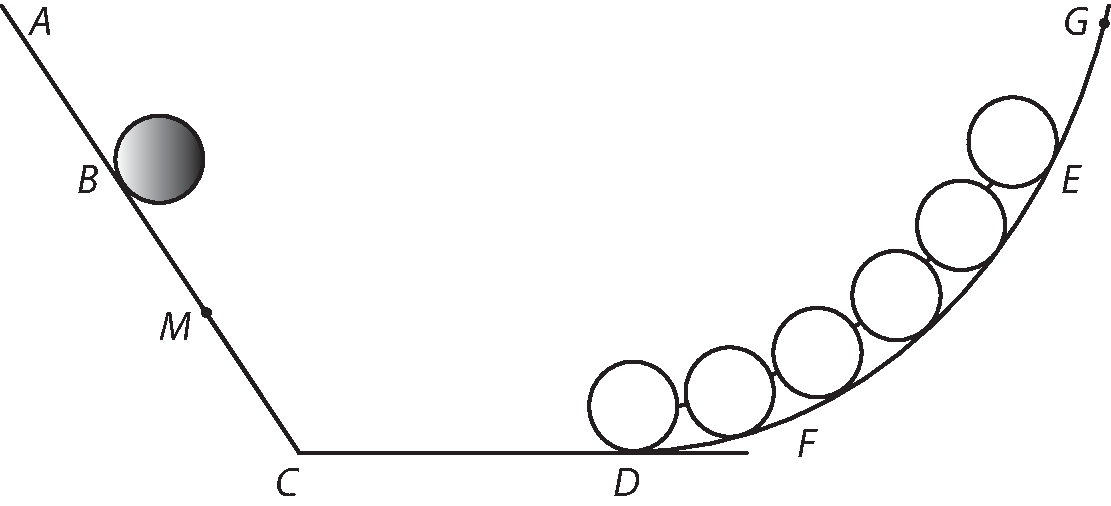
\includegraphics[trim = 0mm -3mm 0mm 0mm, clip, width=0.75\textwidth]{images/LH037,04_061r-d2.pdf}\\
\noindent \centering [\textit{Fig. 2}]
\pend
\newpage
%\vspace*{1em}
\pstart
Si causa\protect\index{Sachverzeichnis}{causa} egit quantum potest; effectus\protect\index{Sachverzeichnis}{effectus} tantum potest quantum causa.
His demonstra\-tis locutiones de communicata potentia\protect\index{Sachverzeichnis}{potentia communicata} poterunt admitti.
\pend
\pstart
Omnis potentia\protect\index{Sachverzeichnis}{potentia} aequalem sibi potentiam\protect\index{Sachverzeichnis}{potentia aequalis} producere potest; in subjecto scilicet habili;
\edtext{et si ad}{\lemma{et si}\Bfootnote{\textbar\ scilicet \textit{gestr.}\ \textbar\ ad \textit{ L}}} 
agendum disposita
\edtext{sit. Nam hoc ipso potentiam\protect\index{Sachverzeichnis}{potentia} metimur, ex quantitate scilicet effectus\protect\index{Sachverzeichnis}{quantitas effectus} quem producere potest.}{\lemma{sit.}\Bfootnote{%
\textit{(1)}\ Ponatur enim potentiam suae 
\textit{(a)}\ minorem 
\textit{(b)}\ aequalem producere non posse, 
\textit{(aa)}\ erit et 
\textit{(bb)}\ et aliquid esse, sequitur
\textit{(2)}\ Nam 
\textit{(a)}\ alioqui 
\textit{(b)}\ hoc [...] potest.
\textit{L}}}
Effectus\protect\index{Sachverzeichnis}{effectus} scilicet non circa rem indifferentem,
sed circa potentiam\protect\index{Sachverzeichnis}{potentia}.
Alioqui enim quidlibet posset infinitum\protect\index{Sachverzeichnis}{infinitum}.
Opus est autem quadam Potentiarum communi mensura;
\edtext{ita corporis potentiam\protect\index{Sachverzeichnis}{potentia corporis} exprimemus si dicemus ipsam producere posse tantam}{\lemma{ita}\Bfootnote{%
\textbar\ dicimus \textit{streicht Hrsg.}\ \textbar\
\textit{(1)}\ tantum posse corporis potentiam
\textit{(2)}\ corporis [...] posse tantam
\textit{L}}}
gravis\protect\index{Sachverzeichnis}{grave} alicujus altitudinem.
Et quod etiam tantam gravis\protect\index{Sachverzeichnis}{grave} ejusdem altitudinem producere poterit,
id tantundem posse videbitur;
cumque grave\protect\index{Sachverzeichnis}{grave} ipsam suam altitudinem possit reproducere;
hinc patet jam hinc effectum\protect\index{Sachverzeichnis}{effectus aequipollens} suae causae\protect\index{Sachverzeichnis}{causa} aequipollere.
Hinc etiam \edtext{demonstratum alium quemlibet}{\lemma{demonstratum}\Bfootnote{%
\textit{(1)}\ aliud quodlibet
\textit{(2)}\ alium quemlibet
\textit{L}}}
\edtext{effectum\protect\index{Sachverzeichnis}{effectus} posse reproducere suam}{\lemma{effectum}\Bfootnote{%
\textit{(1)}\ suam
\textit{(2)}\ posse reproducere suam
\textit{L}}}
\edtext{causam\protect\index{Sachverzeichnis}{causa}, nam}{\lemma{causam,}\Bfootnote{%
\textit{(1)}\ quoniam
\textit{(2)}\ enim
\textit{(3)}\ nam
\textit{L}}}
aequalium potentiarum\protect\index{Sachverzeichnis}{potentia aequalis} effectus sunt
\edtext{aequales\protect\index{Sachverzeichnis}{effectus aequalis}. Sit}{\lemma{aequales}\Bfootnote{%
\textit{(1)}\ ; et
\textit{(2)}\ . Sit
\textit{L}}}
potentia\protect\index{Sachverzeichnis}{potentia} $\displaystyle A$. effectus\protect\index{Sachverzeichnis}{effectus} $\displaystyle B$,
\edtext{qui sit productio}{\lemma{qui sit}\Bfootnote{%
\textit{(1)}\ gravis\protect\index{Sachverzeichnis}{grave} rep
\textit{(2)}\ reproductio
\textit{(3)}\ productio
\textit{L}}}
\edtext{altitudinis[,] tertius}{\lemma{altitudinis[,]}\Bfootnote{%
\textit{(1)}\ se
\textit{(2)}\ tertius
\textit{L}}}
effectus\protect\index{Sachverzeichnis}{effectus} ipsius $\displaystyle A$,
ope $\displaystyle B$. appelletur $\displaystyle BC$,
qui sit reproductio altitudinis.
Sit alius effectus diversus ipsius $\displaystyle A$, nempe $\displaystyle E$.
\edtext{et effectus\protect\index{Sachverzeichnis}{effectus} $\displaystyle E$, sit $\displaystyle D$.}{\lemma{et effectus $\displaystyle E$, sit $\displaystyle D$.}\Bfootnote{\textit{erg. L}}}
ajo ante omnia $\displaystyle E$ posse producere
$\displaystyle D \sqcap BC$.
nam $\displaystyle E \sqcap B$.
quia effectus\protect\index{Sachverzeichnis}{effectus} ejusdem causae\protect\index{Sachverzeichnis}{causa}[,]
aequalium autem potentiarum\protect\index{Sachverzeichnis}{potentia aequalis} aequales effectus\protect\index{Sachverzeichnis}{effectus aequalis},
ergo $\displaystyle D$ effectus ipsius $\displaystyle E$
et $\displaystyle BC$ effectus ipsius $\displaystyle B$ aequales\protect\index{Sachverzeichnis}{effectus aequalis}.
Est autem $\displaystyle BC \sqcap B$.
ergo $\displaystyle D \sqcap B$.
Jam $\displaystyle B \sqcap E$.
ergo $\displaystyle D \sqcap E$.
Unde elaterium\protect\index{Sachverzeichnis}{elaterium} etiam se retendere potest perfecte,
aliaque res quaecunque producere statum,
qui tantundem possit quantum ipsa.
Sed haec demonstratio supponit aliunde demonstratum,
quod corpus grave\protect\index{Sachverzeichnis}{corpus grave} descendens posito rigore accelerationis\protect\index{Sachverzeichnis}{acceleratio},
ad eandem altitudinem resurgat.
Nec alio \edtext{opus fuit axiomate\protect\index{Sachverzeichnis}{axioma},}{\lemma{opus fuit}\Bfootnote{\textbar\ opus \textit{streicht Hrsg.} \textbar\ \ axiomate \textit{ L}}}
quam \edtext{hoc[:] earundem potentiarum\protect\index{Sachverzeichnis}{potentia}}{\lemma{hoc[:]}\Bfootnote{%
\textit{(1)}\ ejusdem poten
\textit{(2)}\ earundem potentiarum
\textit{L}}}
effectus sunt aequales\protect\index{Sachverzeichnis}{effectus aequalis}.
Effectus\protect\index{Sachverzeichnis}{effectus} autem et ipsi a potentia\protect\index{Sachverzeichnis}{potentia} quam continent aestimantur.
Unde cum di$\displaystyle\langle$citur$\displaystyle\rangle$
aequales esse effectus\protect\index{Sachverzeichnis}{effectus aequalis}, intelligitur aequalis esse potentiae;
et dici poterat, aequalium potentiarum\protect\index{Sachverzeichnis}{potentia aequalis}
effectus pleni\protect\index{Sachverzeichnis}{effectus plenus} sunt aequipollentes\protect\index{Sachverzeichnis}{effectus aequipollens}.
Ex hoc axiomate\protect\index{Sachverzeichnis}{axioma} etiam nulla re aliunde ascita videb$\displaystyle\langle$itur$\displaystyle\rangle$
demonstrari posse, quod effectus sit
\edtext{causae\protect\index{Sachverzeichnis}{causa} aequipollens\protect\index{Sachverzeichnis}{effectus equipollens}}{\lemma{causae}\Bfootnote{%
\textit{(1)}\ aequalis
\textit{(2)}\ aequipollens
\textit{L}}},
quia $\displaystyle E$ et $\displaystyle D$ sunt effectus pleni\protect\index{Sachverzeichnis}{effectus plenus} ejusdem $\displaystyle\langle$causae.$\displaystyle\rangle$
[61~v\textsuperscript{o}]
\pend
\newpage
\count\Bfootins=1500
\pstart
\begin{wrapfigure}{l}{0.5\textwidth}
\vspace{-4mm}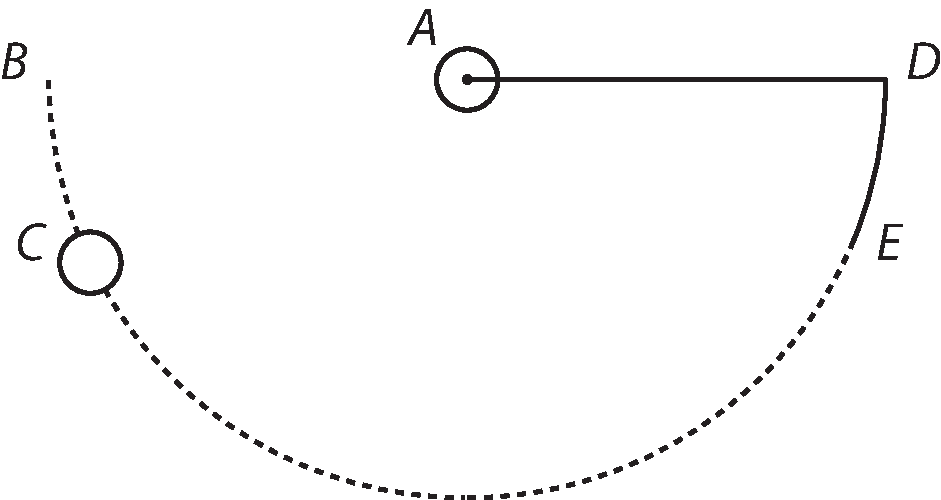
\includegraphics[trim = 0mm -3mm -5mm 0mm, clip, width=0.49\textwidth]{images/LH037,04_061v-d1.pdf}\\
\noindent
\centering
[\textit{Fig. 3}] % \caption{Bildbeschreibung}
\end{wrapfigure}
%%
Et mirum sane axioma\protect\index{Sachverzeichnis}{axioma} est, quod afferimus;
quolibet momento temporis ab eadem causa\protect\index{Sachverzeichnis}{causa}
aequalem semper potentiam\protect\index{Sachverzeichnis}{potentia aequalis} produci.
Sit machina\protect\index{Sachverzeichnis}{machina} quaelibet in motu constituta,
ajo aequali semper vi ad eam sistendam esse opus,
modo scilicet totam vim suam jam possideat;
aliud enim est si ipsa potentia\protect\index{Sachverzeichnis}{potentia} augeri possit,
ut si nova ei pondera\protect\index{Sachverzeichnis}{pondus} appendi possint;
aut si inferius possint descendere.
Hinc si lapis aliquis a summo ad quantam potest altitudinem descenderit,
tunc si continuet suas reciprocationes, aequali semper vi opus erit ad ipsum sistendum;
imo non ita res exprimenda sed hoc modo[:]
si corpus $\displaystyle C$ ex $\displaystyle B$, et $\displaystyle DE$ ex $\displaystyle D$,
descendentia alicubi aequivaleant, ubilibet aequivalebunt.
Nostrum autem \edtext{axioma\protect\index{Sachverzeichnis}{axioma} intelligitur,}{\lemma{axioma}\Bfootnote{%
\textit{(1)}\ tale errat;
\textit{(2)}\ intelligitur,
\textit{L}}}
modo nova absit actio\protect\index{Sachverzeichnis}{actio}, hinc ubi grave\protect\index{Sachverzeichnis}{grave} post descensum\protect\index{Sachverzeichnis}{descensus} in planum horizontale pervenit,
nihil amplius conferet vis gravitatis\protect\index{Sachverzeichnis}{vis gravitatis}, adeoque eandem semper vim habebit.
\pend
\pstart
Caeterum si quis neget hanc consequentiam[:]
si sint $\displaystyle A$. $\displaystyle E$. $\displaystyle D$.
et $\displaystyle A$ causa\protect\index{Sachverzeichnis}{causa} $\displaystyle E$, et $\displaystyle E$ causa $\displaystyle D$,
aequipollere $\displaystyle E$ et $\displaystyle D$,
quippe Effectus\protect\index{Sachverzeichnis}{effectus} ejusdem causae\protect\index{Sachverzeichnis}{causa} $\displaystyle A.$
ei ostendendum, quodsi minor effectus $\displaystyle D$ quam $\displaystyle E$,
utique quia tempus $\displaystyle AE$, quod
\edtext{inter $\displaystyle A$ et Effectum\protect\index{Sachverzeichnis}{effectus}}{\lemma{inter}\Bfootnote{%
\textit{(1)}\ effectum
\textit{(2)}\ $\displaystyle A$ et Effectum
\textit{L}}}
$\displaystyle E$ intercedit in infinitas\protect\index{Sachverzeichnis}{infinitas} dividi potest partes;
posse interponi effectus infinitos\protect\index{Sachverzeichnis}{effectus infinitus} priores ipso
\begin{wrapfigure}[12]{l}{0.4\textwidth}
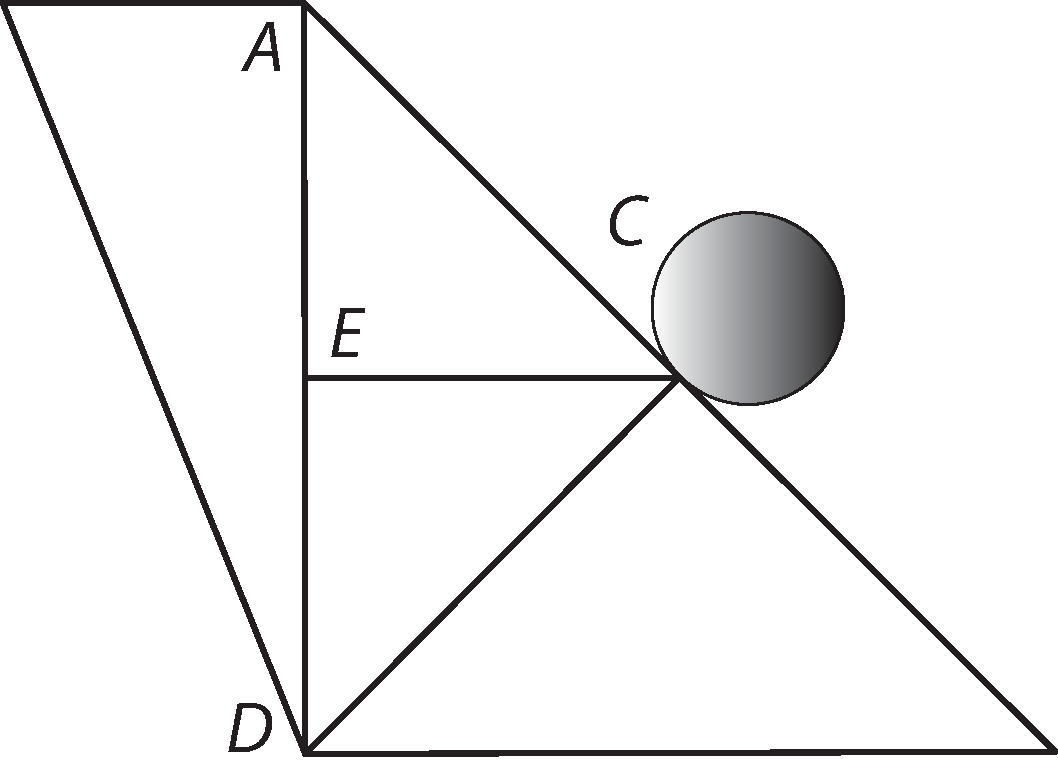
\includegraphics[trim = 0mm -3mm -5mm 0mm, clip, width=0.4\textwidth]{images/LH037,04_061v-d2.pdf}\\
\noindent
\centering
[\textit{Fig. 4}] % \caption{Bildbeschreibung}
\end{wrapfigure} 
effectu $\displaystyle E$.
quodsi ergo sola per se distantia effectus a causa\protect\index{Sachverzeichnis}{causa} diminuit
\edtext{vel auget}{\lemma{vel auget}\Bfootnote{\textit{erg. L}}} effectum\protect\index{Sachverzeichnis}{effectus};
demonstrari poterit, diminui proportionaliter pro ratione elongationis;
neque enim ulla alia relatio determinata fingi potest,
quia hic nulla particularis consideratio;
itaque alterutrum sequeretur,
vel effectum fore infinitum\protect\index{Sachverzeichnis}{effectus infinitus} relatione ad aliquam causam\protect\index{Sachverzeichnis}{causa},
vel contra eodem modo demonstrari potest absurditas,
si ponatur effectus\protect\index{Sachverzeichnis}{effectus} \edtext{in duplicata ratione}{\lemma{in}\Bfootnote{%
\textit{(1)}\ proportione qua
\textit{(2)}\ duplicata ratione
\textit{L}}}
elongationum, vel in reciproca vel ut differentiae.
Sed nec in reciproca potest esse,
foret \edtext{enim alicubi}{\lemma{enim}\Bfootnote{%
\textit{(1)}\ mox
\textit{(2)}\ alicubi
\textit{L}}}
causa infinita\protect\index{Sachverzeichnis}{causa infinita} vel contra, etsi alterum nunquam.
Restant tantum curvae,
quae in unam tantum partem habent
\edtext{asymptoton\protect\index{Sachverzeichnis}{asymptotos}[,] secundum quas fingi posset incrementum vel decrementum, sed}{\lemma{asymptoton[,]}\Bfootnote{%
\textit{(1)}\ sed
\textit{(2)}\ secundum [...] decrementum, sed
\textit{L}}}
eae specialibus utique opus habent naturis.
Et generalis sufficit demonstratio nobis,
sine curvarum speciali consideratione;
quod scilicet[,] in summa generalitate, nulla alia
\edtext{potest haberi relatio}{\lemma{potest}\Bfootnote{%
\textit{(1)}\ consideratio
\textit{(2)}\ haberi relatio
\textit{L}}}
quam proportio simplex,
cum sola distantia temporis sine ullo alio contribuente,
dicatur diminuere effectum\protect\index{Sachverzeichnis}{effectus} vel augere.
\pend
\pstart
Est et alia fortissima ratio, quod scilicet effici potest,
ut idem effectus\protect\index{Sachverzeichnis}{effectus} longiore post tempore sequatur[,]
quare si sola temporis differentia causa\protect\index{Sachverzeichnis}{causa} est,
utique idem sibi ipsi inaequale erit,
poterit tamen responderi
multitudinem effectuum\protect\index{Sachverzeichnis}{effectus} interjectorum[,] non ipsum per se tempus esse in
\edtext{causa; imo non multitudinem}{\lemma{causa;}\Bfootnote{%
\textit{(1)}\ item, cum mu
\textit{(2)}\ imo non multitudinem
\textit{L}}}
solum sed quantitatem\protect\index{Sachverzeichnis}{quantitas effectus}.
Alio uti licebit argumento;
nimirum, opus esse quadam incrementi vel diminutionis
\edtext{uniformitate\protect\index{Sachverzeichnis}{uniformitas}; vel in}{\lemma{uniformitate;}\Bfootnote{%
\textit{(1)}\ ut si
\textit{(2)}\ vel in
\textit{L}}}
re recte expensa quaeritur longitudo ipsarum $\displaystyle M$. $\displaystyle N$. $\displaystyle P$.
seu natura curvae $\displaystyle M$. $\displaystyle N$. $\displaystyle P$. 
cum in infinitum\protect\index{Sachverzeichnis}{infinitum} retro eadem semper futura sit curva;
et, quod demonstrare poterimus in $\displaystyle A$. $\displaystyle E$. $\displaystyle D$,
pari jure initio potuerimus dicere de $\displaystyle (A)$. $\displaystyle (E)$. $\displaystyle (D)$[;]
ideo curva $\displaystyle MNP$. curvae $\displaystyle (M)(N)(P)$ per omnia congruet,
seu erit recta,
\edtext{ut si curva}{\lemma{ut si}\Bfootnote{%
\textit{(1)}\ alicubi curva
\textit{(2)}\ curva
\textit{L}}} sit;
erit utique tangens ejus talis,
ut certum aliquem angulum faciat ad $\displaystyle AED$.
\pend
\pstart
Item aliter: quoniam non est determinatum,
quomodo sumi debeat una ex rectis,
\edtext{ut $\displaystyle AM$,
tunc vero reliquae omnes $\displaystyle EN$, $\displaystyle DP$ fiant etiam minores;
et vero nulla sit linea $\displaystyle MNP$, in qua}{\lemma{ut $\displaystyle AM$,}\Bfootnote{%
\textit{(1)}\ et vero nulla est linearum in qu
\textit{(2)}\ tunc [...] in qua
\textit{L}}}
proportionalia fiant omnia quamcunque sumas $\displaystyle AM$, praeterquam si sit recta;
ideo necesse est $\displaystyle MNP$ esse rectam;
eadem non est inclinata ad $\displaystyle AD$,
alioquin ei alicubi occurreret,
et aliquando effectus
\edtext{foret infinite parvus\protect\index{Sachverzeichnis}{effectus infinite parvus}; ut}%
{\lemma{foret}\Bfootnote{%
\textbar\ infinitus \textit{gestr.}
\textbar\ vel \textit{streicht Hrsg.}
\textbar\ infinite parvus;
\textit{(1)}\ quoniam
\textit{(2)}\ ut
\textit{L}}}
in $\displaystyle Q$.
Sed tunc idem rursus absurdum,
nam alio longiore sumto $\displaystyle M$ initio, idem $\displaystyle Q$ seu effectus infinite parvus\protect\index{Sachverzeichnis}{effectus infinite parvus}
longius differretur,
ergo necesse est rectam $\displaystyle MNP$ esse
\edtext{parallelam ipsi $\displaystyle AQ$. ita enim nihil referet}{\lemma{parallelam}\Bfootnote{%
\textit{(1)}\ , ita enim nihil referet
\textit{(2)}\ ipsi [...] referet
\textit{L}}}
quae initio sumatur $\displaystyle AM$.
Magni momenti videntur esse hujusmodi universales ratiocinationes.
Certe si inclinata
\edtext{esset, recta una ad aliam; jam dudum}{\lemma{esset,}\Bfootnote{%
\textit{ (1) }\ tum jam dudum
\textit{ (2) }\ recta [...] dudum
\textit{ L}}}
infinite abhinc eam attigisset, cum quaelibet causa\protect\index{Sachverzeichnis}{causa} habeat
effectus ante ipsam infinitos\protect\index{Sachverzeichnis}{effectus infinitus}.
\pend
%\vspace{1em}
\newpage% PR: Rein provisorisch!
\pstart
\noindent
\centering
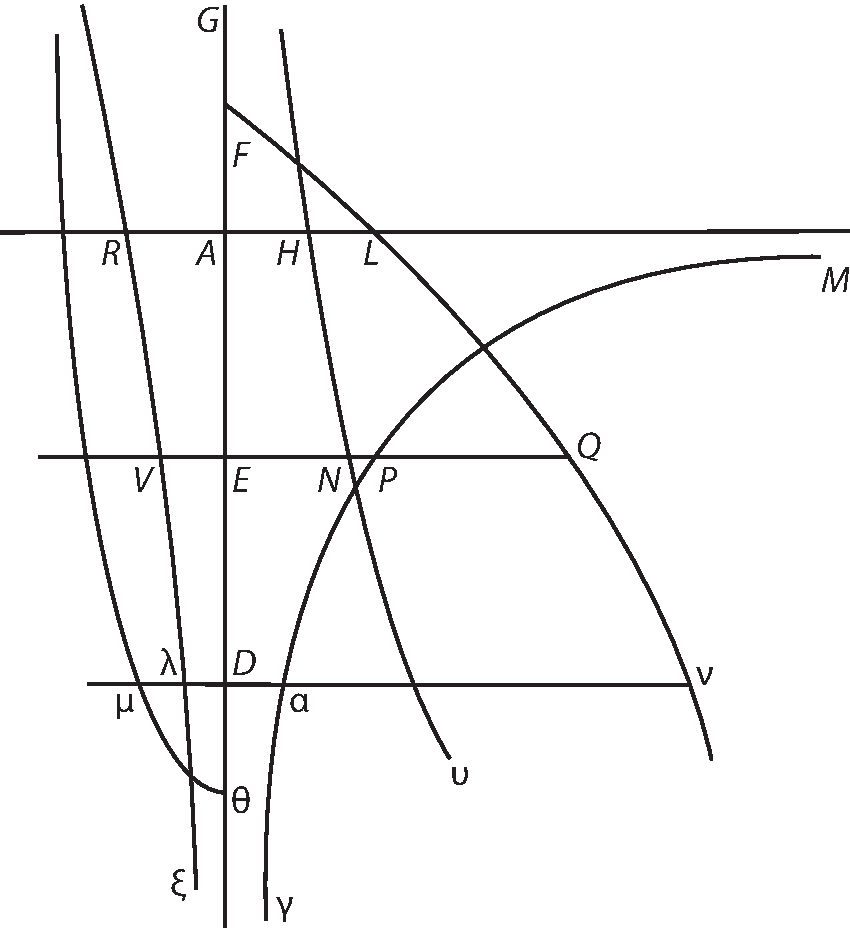
\includegraphics[trim = 0mm -3mm 0mm 0mm, clip, width=0.58\textwidth]{images/LH037,04_061v-d3.pdf}\\
\noindent \centering [\textit{Fig. 5}]
\pend
\pstart
\vspace{1em}
\begin{minipage}[t]{0.345\textwidth}
\hspace*{-5mm}
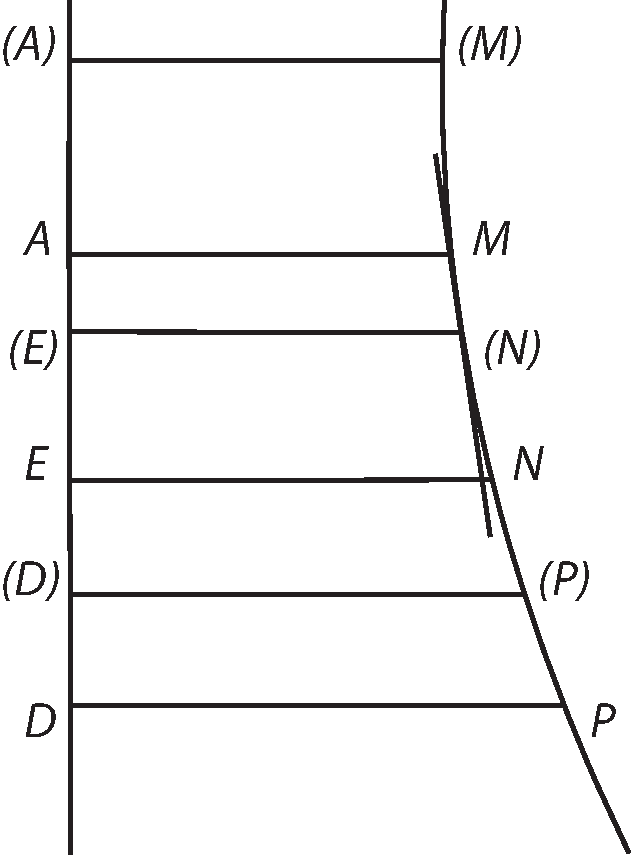
\includegraphics[trim = 0mm -3mm 0mm 0mm, clip, width=1\textwidth]{images/LH037,04_061v-d4.pdf}
\noindent \centering [\textit{Fig. 6}]
\end{minipage}
\hspace*{21,9mm}
\begin{minipage}[t]{0.40\textwidth}
\hspace*{-5mm}
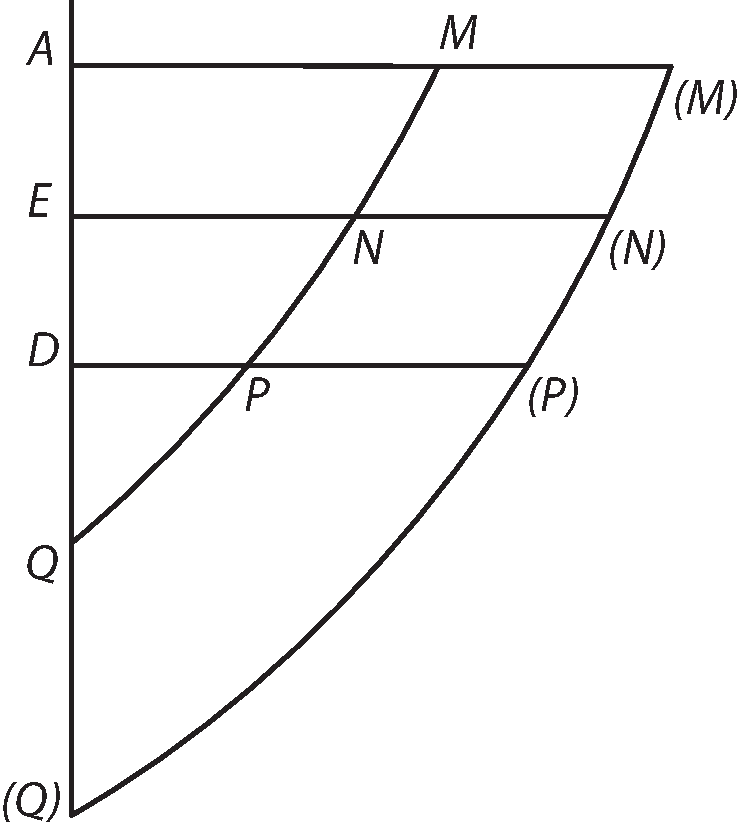
\includegraphics[trim = 0mm -3mm 0mm 0mm, clip, width=1\textwidth]{images/LH037,04_061v-d5.pdf}
\noindent \centering [\textit{Fig. 7}]
\end{minipage}
%\vspace*{0.5em}
\pend
\newpage
%%%%
%%%%
%\pstart
%Item aliter: quoniam non est determinatum,
%quomodo sumi debeat una ex rectis,
%\edtext{ut $\displaystyle AM$,
%tunc vero reliquae omnes $\displaystyle EN$, $\displaystyle DP$ fiant etiam minores;
%et vero nulla sit linea $\displaystyle MNP$, in qua}{\lemma{ut $\displaystyle AM$,}\Bfootnote{%
%\textit{(1)}\ et vero nulla est linearum in qu
%\textit{(2)}\ tunc [...] in qua
%\textit{L}}}
%proportionalia fiant omnia quamcunque sumas $\displaystyle AM$, praeterquam si sit recta;
%ideo necesse est $\displaystyle MNP$ esse rectam;
%eadem non est inclinata ad $\displaystyle AD$,
%alioquin ei alicubi occurreret,
%et aliquando effectus
%\edtext{foret infinite parvus\protect\index{Sachverzeichnis}{effectus infinite parvus}}{\lemma{foret}\Bfootnote{%
%\textbar\ infinitus\protect\index{Sachverzeichnis}{effectus infinitus}\ \textbar\ vel \textit{streicht Hrsg.}\ \textbar\ \textit{gestr.}\ \textbar\ infinite parvus
%\textit{L}}}\edtext{; ut}{\lemma{parvus;}\Bfootnote{%
%\textit{(1)}\ quoniam
%\textit{(2)}\ ut
%\textit{L}}}
%in $\displaystyle Q$.
%Sed tunc idem rursus absurdum,
%nam alio longiore sumto $\displaystyle M$ initio, idem $\displaystyle Q$ seu effectus infinite parvus\protect\index{Sachverzeichnis}{effectus infinite parvus}
%longius differretur,
%ergo necesse est rectam $\displaystyle MNP$ esse
%\edtext{parallelam ipsi $\displaystyle AQ$. ita enim nihil referet}{\lemma{parallelam}\Bfootnote{%
%\textit{(1)}\ , ita enim nihil referet
%\textit{(2)}\ ipsi [...] referet
%\textit{L}}}
%quae initio sumatur $\displaystyle AM$.
%Magni momenti videntur esse hujusmodi universales ratiocinationes.
%Certe si inclinata
%\edtext{esset, recta una ad aliam; jam dudum}{\lemma{esset,}\Bfootnote{%
%\textit{ (1) }\ tum jam dudum
%\textit{ (2) }\ recta [...] dudum
%\textit{ L}}}
%infinite abhinc eam attigisset, cum quaelibet causa\protect\index{Sachverzeichnis}{causa} habeat
%effectus ante ipsam infinitos\protect\index{Sachverzeichnis}{effectus infinitus}.
%\pend
\pstart
%\begin{wrapfigure}[5]{l}{0.5\textwidth}
\centering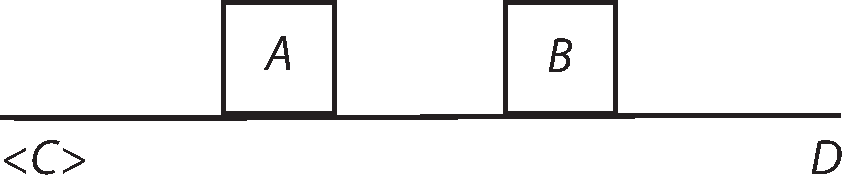
\includegraphics[trim = 0mm -1mm 0mm 0mm, clip, width=0.48\textwidth]{images/LH037,04_061v-d6.pdf}\\
\noindent
\centering
[\textit{Fig. 8}] % \caption{Bildbeschreibung}
%\end{wrapfigure}
%%
\pend
\vspace{1.5em}
\pstart
Adjicienda \setline{1}ratiocinatio de quantitate viae, seu loci successivi.
Item examinandum an aliquid solidi subsit huic ratiocinationi meae veteri.
Corpora $\displaystyle A$. $\displaystyle B$ eadem celeritate\protect\index{Sachverzeichnis}{celeritas} sibi occurrunt,
ajo reditura eadem qua venere celeritate;
supposito conatum impossibilem\protect\index{Sachverzeichnis}{conatus impossibilis} evanescere.
In momento concursus\protect\index{Sachverzeichnis}{concursus}, $\displaystyle A$ accipit
\edtext{a $\displaystyle B$ conatum}{\lemma{a $\displaystyle B$}\Bfootnote{%
\textit{(1)}\ celeritatem
\textit{(2)}\ conatum
\textit{L}}}
a $\displaystyle D$ versus $\displaystyle C$ eundi;
et dat ipsi [$\displaystyle B$]\edtext{}{\Bfootnote{$\displaystyle D$ \textit{\ L \"{a}ndert Hrsg.}}}
conatum\protect\index{Sachverzeichnis}{conatus} a $\displaystyle C$ versus $\displaystyle D$ eundi;
habent ergo ambo
\edtext{simul utrumque}{\lemma{simul}\Bfootnote{%
\textit{(1)}\ ipsum
\textit{(2)}\ utrumque
\textit{L}}} conatum;
eum quem habebant et quem accepere;
\edtext{conatus impossibilis\protect\index{Sachverzeichnis}{conatus impossibilis} effectu\protect\index{Sachverzeichnis}{effectus} caret.}{\lemma{conatus}\Bfootnote{%
\textbar\ autem \textit{gestr.}\ \textbar\ impossibilis
\textit{(1)}\ evanescit
\textit{(2)}\ effectu caret
\textit{L}}}
Est autem impossibile $\displaystyle A$ ire versus $\displaystyle D$,
et \edtext{simul}{\lemma{simul}\Bfootnote{\textit{erg. L}}}
$\displaystyle B$ ire versus $\displaystyle C$ ob corporum impenetrabilitatem\protect\index{Sachverzeichnis}{impenetrabilitas}. %<marg-1>
Ergo restabit in $\displaystyle A$ tantum conatus\protect\index{Sachverzeichnis}{conatus} redeundi versus $\displaystyle C$,
et in $\displaystyle B$ \edtext{conatus redeundi}{\lemma{conatus}\Bfootnote{%
\textit{(1)}\ eundi
\textit{(2)}\ redeundi
\textit{L}}}
versus $\displaystyle D$.
Videtur hinc porro sequi quod etsi inaequali venerint celeritate\protect\index{Sachverzeichnis}{celeritas}[,]
modo ipsa sint aequalia[,] permutatis eant celeritatibus.
Sed si inaequalia ostendendum habendam magnitudinis rationem.
[62~r\textsuperscript{o}]
\pend
\pstart
Si duo conatus incompossibiles\protect\index{Sachverzeichnis}{conatus incompossibilis} aequales componantur,
nil refert, quod unus fortior alio,
jam enim fecere effectum\protect\index{Sachverzeichnis}{effectus} suum,
quare non est quaestio de eorum fortitudine\protect\index{Sachverzeichnis}{fortitudo}.
Conatus\protect\index{Sachverzeichnis}{conatus} duo,
ut idem corpus simul tendat in diversas partes[,]
inter se possunt componi;
non vero ut duo corpora simul tendant in eundem locum,
seu se penetrent.
Nihil refert \edtext{[utrum]}{\lemma{utrum}\Bfootnote{\textit{erg. Hrsg.}}}
duo mobilia\protect\index{Sachverzeichnis}{mobile} ad se invicem ferantur
an vero alterum quiescat alterum moveatur;
poterit et celeritas\protect\index{Sachverzeichnis}{celeritas} inter ea dividi aequaliter.
Ostendendum est semper prodire idem.
Nulla est destructio in conatibus\protect\index{Sachverzeichnis}{conatus};
nam cum duo inaequalis fortitudinis\protect\index{Sachverzeichnis}{fortitudo} concurrunt
non ideo fortior destruit debiliorem ullo modo,
sed uterque durat et componuntur si unum moveatur alterum quiescat,
ex his etiam sequitur motum vim quiescentis accipere, et ei dare suam.
Examinandum tamen, nam in hoc difficultas.
Videtur enim majus non semper in loco minoris consistere eique suam vim dare,
quod tamen ex his positis sequeretur.
Haec ergo ratiocinatio forte non exacta.
Si haec vera essent corpus maximum a minimo sisteretur,
sed minimum hoc reciperet totam vim majoris adeoque maxima moveretur celeritate\protect\index{Sachverzeichnis}{celeritas}.
Haec ergo exactius examinanda;
et difficultas etiam ex eo, quod ista videntur eventura, indifferenter;
salvo semper eodem principio de vi prima manente.
An forte si nullum esset Elaterium\protect\index{Sachverzeichnis}{elaterium} sed durities\protect\index{Sachverzeichnis}{durities} summa,
ista evenirent? Videndum.
\pend
\pstart
In Elastico corpore\protect\index{Sachverzeichnis}{corpus elasticum} video multa conjungenda,
et rem subtilius examinandam,
conatus penetrationis\protect\index{Sachverzeichnis}{conatus penetrationis} seu quo corpus alteri cedit,
effectum\protect\index{Sachverzeichnis}{effectus} suum hic sortitur;
non ex toto tamen,
fit enim quaedam lucta inter corporis resistentiam\protect\index{Sachverzeichnis}{resistentia corporis}
\edtext{ad transformationem}{\lemma{ad}\Bfootnote{%
\textit{(1)}\ flexum
\textit{(2)}\ transformationem
\textit{L}}},
et inter ipsum motum unius ad alterum,
ubi ad eum venere compressionis\protect\index{Sachverzeichnis}{compressio} statum,
\edtext{ut tota}{\lemma{ut}\Bfootnote{\textbar\ non amplius \textit{gestr.}\ \textbar\ tota \textit{L}}}
vis consumta sit;
tunc vis quae in corpore est, se restituendi, suas partes agit.
Opus ista habent adhuc exacta discussione.
Et determinandum est,
quae sit magnitudo corporis\protect\index{Sachverzeichnis}{magnitudo corporis},
ubi a corpore parvo sisti desinit.
\pend
\vspace*{2em}
\pstart
\noindent
[\textit{In der unteren linken Ecke von Bl. 61~v\textsuperscript{o}, durch eine Linie umrahmt}:]
\pend
\vspace*{0.5em}
\pstart
\noindent
$\displaystyle\langle$--- ---$\displaystyle\rangle$ mirum eadem praestare
$\displaystyle\langle$--- ---$\displaystyle\rangle$ quae duritiem\protect\index{Sachverzeichnis}{durities}, quia posita vi elaterii\protect\index{Sachverzeichnis}{vis elaterii}
$\displaystyle\langle$--- ---$\displaystyle\rangle$ in statum priorem sequitur
$\displaystyle\langle$--- ---$\displaystyle\rangle$ore effectum\protect\index{Sachverzeichnis}{effectus},
$\displaystyle\langle$--- ---$\displaystyle\rangle$ ab eo no%
$\displaystyle\langle$--- ---$\displaystyle\rangle$
\pend